\documentclass[authoryearcitations]{UoYCSproject}
\usepackage{todonotes}

\author{Joshua Goodwin}
\title{Layout of arguments in the Artoo tool}
% \date{}
\supervisor{Fiona Polack}
\BEng

\wordcount{?}

% \includes{Appendices \ref{cha:usefulpackages}, \ref{cha:gotchas} and
  % \ref{cha:deptfac}}

% \excludes{\autoref{cha:quoteex}}

\abstract{}

% \dedication{To}

% \acknowledgements{
%   I would like to thank
% }

\begin{document}

\maketitle

% \listoffigures
% \listoftables
% \renewcommand*{\lstlistlistingname}{List of Listings}
% \lstlistoflistings

% \cleardoublepage

% \part{Preliminaries}
% \label{sec:start}
% \thispagestyle{empty}\cleardoublepage

%%%%%%%%%%%%%%%%%%%%%%%%%%%%%%%%%%%%%%%%%%%%%%%%%%%%%%%%%%%

\chapter{Introduction?}


\section{The Goal Structuring Notation}

The Goal Structuring Notation (GSN) is a graphical agumentation notation.
It allows logical arguments - in particular, safety arguments, which \ldots  - to be represented explicitly, in a much clearer way than textual arguments allow.

GSN arguments are directed, multivariate \todo{I think}, hierachical graphs.

An argument begins with a single, main goal or claim\todo{two words used interchangably\ldots}. rectangle

Nodes within GSN arguments contain text, and represent ``claims, strategies, evidence, and context/assumption/justification annotations'';
edges represent relationships between these.

\begin{description}
    \item[Goal/claim]
    a statement that can be assessed to be true or false
    \item[Strategy]
\end{description}

\begin{figure}
    \centering
    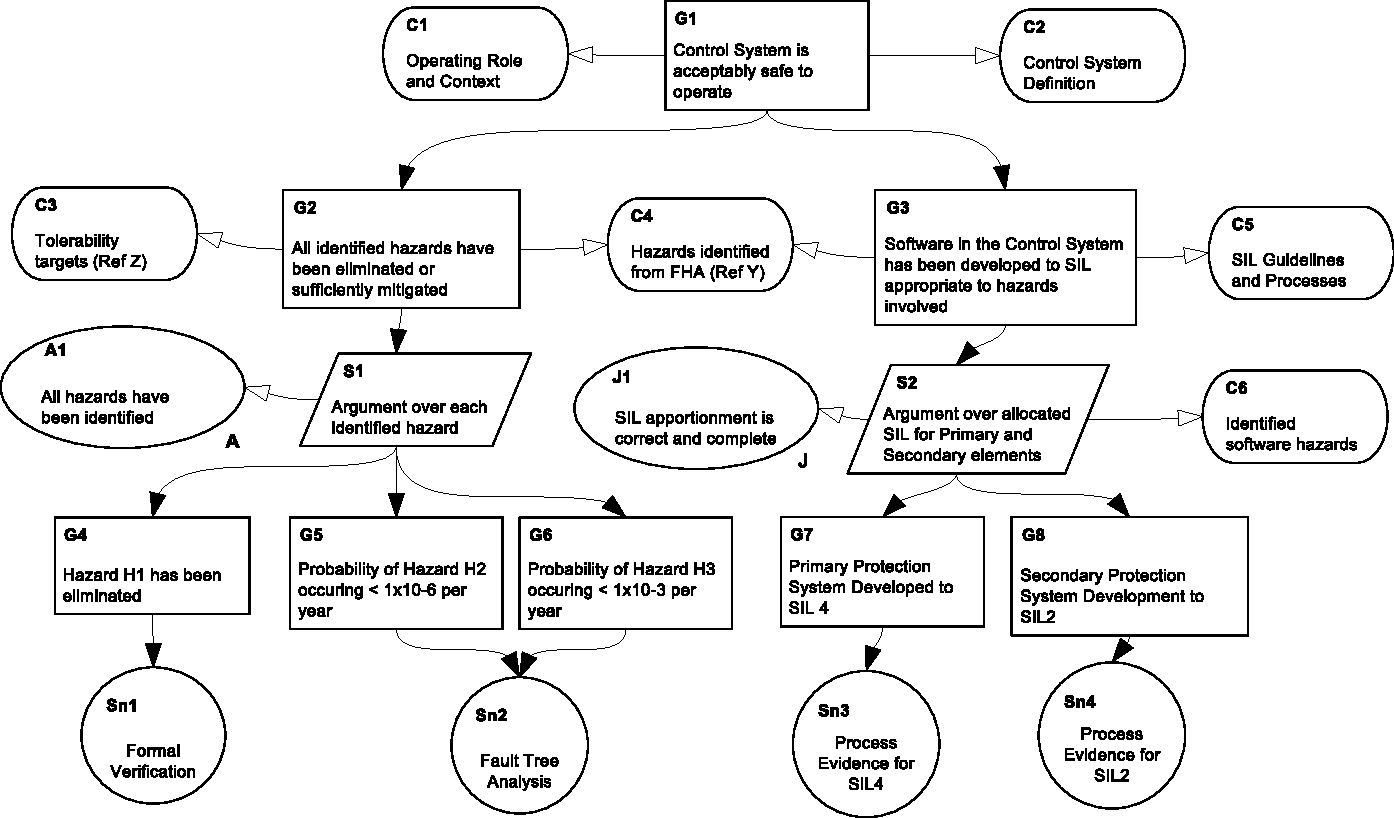
\includegraphics[width=\textwidth]{example_argument.pdf}
    \caption{An example argument, from the GSN specification}
\end{figure}

\ldots

other notations: Connt

\section{Artoo}

Artoo (Argumentation Tool) is a web-based tool intended for drawing GSN arguments.

\ldots

other tools also exist for drawing GSN argments.

\begin{figure}
    \centering
    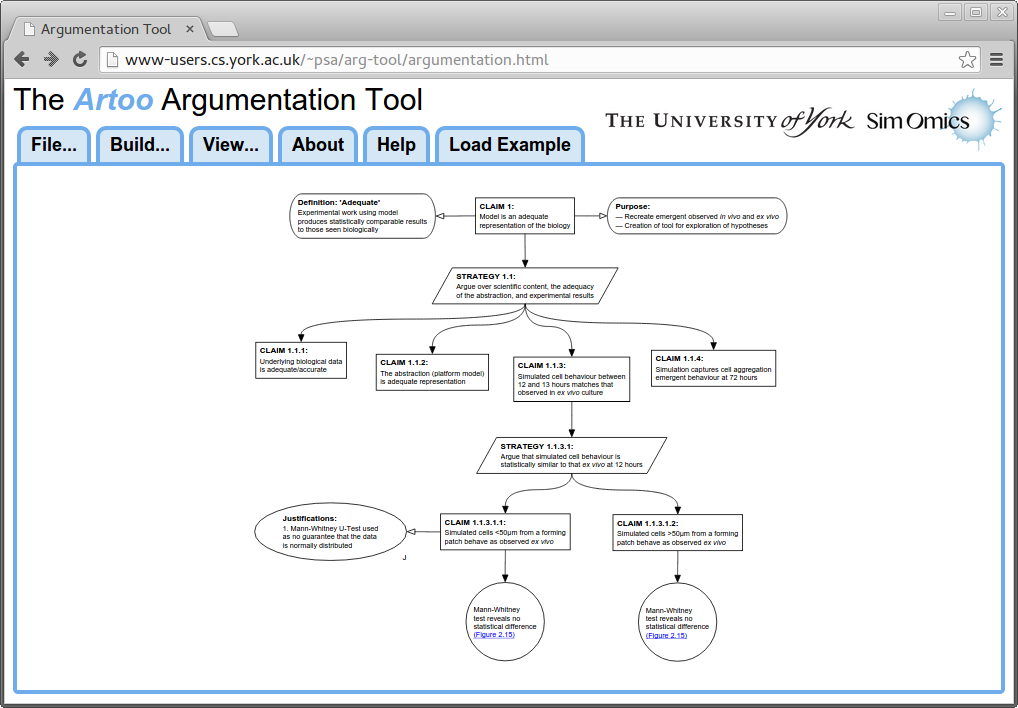
\includegraphics[width=\textwidth]{graphics/artoo_screenshot.png}
    \caption{The Artoo tool, displaying an argument }
\end{figure}

\todo{use the same argument as in the naked dexample?}

\section{[what I'm going to do]}

This [report/project/thing] will \ldots

    \begin{enumerate}
        \item \begin{itemize}
            \item ,
        \end{itemize}
    \end{enumerate}

\subsection{Problem definition?}

Input:

[GSN arguments are directed, multivariate \todo{I think} graphs.]



\subsection{Problem definition?}

Artoo also allows the drawing of invalid GSN argments ...
if the graph layout [thing] is to be executed every time the graph is edited, then it must accept these .
If the algorithm [is exposed to the user by a] button, then there is the poissibility.

\subsubsection{\ldots}

Already, Artoo only works a limited set of web browsers: recent versions of \ldots
The features added in this project will not [interface] with the browser in any new way -- only needing to change the position of nodes \ldots



\chapter{Literature review}

\section{A brief history}

In 1736, \citet{euler} solved the Seven Bridges of Ka\"{o}nigsberg problem by drawing a graph.
\citet{ismail2009some}
\todo{a strange paper to choose. perhaps multiple citations?}
pinpoint his use of this method as the birth of graph theory.

In 1963, \citet{tutte} popularised the problem of graph drawing when he presented 

who showed that polyhedral graphs may be drawn in the plane with all faces convex by fixing the vertices of the outer face of a planar embedding of the graph into convex position, placing a spring-like attractive force on each edge, and letting the system settle into an equilibrium

Perhaps his most relevant finding was that 

In the same year, \citet{Knuth63} described a system for drawing flowcharts that describe algorithms. \citet{battista} \todo{find out page number!} says this is [the first example of an algorithm for visualising information] although \citeauthor{Knuth63} cites earlier work done on a similar system by \citet{haibt1959}.




\ldots

\citet{huang2007effects} divide graphs into two groups: abstract graphs and domain graphs.
GSN arguments fall into the latter category \ldots  therefore \ldots
\todo{I don't think this is widely agreed upon}


\section{What makes a good graph layout?}

Speed is one 

The Gestalt theories of visual perception, developed from a wider Gestalt theory of the mind  \ldots German psychologists \ldots the Berlin School \ldots inform  \ldots 

The principle 

Some studies have tried \ldots cognitive effects [Purchase et al?]

\subsection{Edge crossings}

There can be many practical motivations for minimising edge crossings.
When P\`{a}l Tur\`{a}n worked in a brick factory during World War II, he wondered about the minumum number of crossings in a graph representing brick kilns, storage sites and the paths between them \ldots
When a graph represents an electrical circuit, 



\section{techniques?}

[gastner 199*]

\subsection{force dire}

\ldots a successor to \citet{tutte} spring embedding

 

\section{[GSN-/Artoo-specific considerations?]}

[move to Requirements?]

The GSN specification citep[section~2.2, pp.~26--27]\{\} gives some guidance on the layout of arguments \ldots

\subsection{Dangling edges}


\subsection{Cycles}

It can be useful to remove directed cycles from the internal representation of a graph (before drawing the edges in the correct, original order) -- for example, in order to assign a rank to each node.
This is achieved by reversing certain edges. \citet{gansner1993} Minimising the 

Undirected cycles can be elimiated by ignoring certain edges altogether to produce a tree.  [citation needed]






\section{A force directed approach}



\chapter{}


\section{[Alternatives to JavaScript]}

Various [things] have been developed in response to percieved shortcomings in JavaScript \ldots

Programs written in the CoffeeScript\footnote{\url{http://coffeescript.org/}} language, designed to be more succinct and with some extra features, can be transcompiled to JavaScript \ldots this is interesting but \ldots

Brython \footnote{\url{http://www.brython.info/}} is a Python 3 interpreter written in JavaScript that can run in a web browser. Haste\footnote{\url{http://haste-lang.org/}}, UHC-JS\footnote{\url{http://uu-computerscience.github.io/uhc-js/}} and GHCJS are compilers from Haskell to JavaScript. 


ASM\footnote{[ASM]} is a strict subset of 

\section{Software development methodologies}

In \citeyear{67poorslop}, \citet{67poorslop} explained ``Why Programming is a Good Medium for Expressing Poorly Understood and Sloppily Formulated Ideas''.
(More recently, [sussman] gave a talk with the same title \todo{\url{http://vimeo.com/12060509}}

\bibliography{report}

% appendices go here

\end{document}